\documentclass[12pt, a4paper]{article}
\usepackage[utf8]{inputenc}
\usepackage[russian]{babel}
\usepackage{ulem}

\usepackage{verbatim}
\usepackage{epigraph}
\usepackage{graphicx}
\usepackage{titlesec}
\newcommand{\sectionbreak}{\clearpage}

\graphicspath{{pictures/}}

\pagestyle{headings}

\title{Информатика}
\date{Май 2019}

\begin{document}

\maketitle

\section{CS102. Объектно-ориентированная парадигма.}

\subsection{Объектно-ориентированное программирование: объектно-ориентированное проектирование, инкапсуляция и скрытие информации; разделение интерфейса и реализации; классы, наследники и наследование; полиморфизм; иерархии классов.}

ООП --- Методология программирования, основанная на представлении программы в виде совокупности объектов, каждый из которых является экземпляром определённого класса, а классы образуют иерархию наследования.

Гради Буч: "Объект обладает состоянием, поведением и индивидуальностью"{}.

Мотивация к созданию --- структуризация кода, сокращение длины кода, улучшение понимания кода, упрощение модификации кода, переиспользования кода.

Основоположник ООП --- Алан Кэй. Сформулировал "биологическую модель". Кэй предложил идею идеального компьютера, который должен функционировать подобно живому организму; каждая "клетка"\ которого должна вести себя в соответствии с другими, чтобы выполнить конечную цель, а также должна уметь функционировать автономно. Кроме того, "клетки"\ должны иметь способность перегруппировывать сами себя для решения другой проблемы или выполнения другой функции.
В течение двух лет, начиная с 1970 года, Алан Кэй работал над языком Smalltalk, который разрабатывался для того, чтобы смоделировать ранее описанную биологическую модель, состоящую из ячеек (или "клеток"{}) и передачи сообщений между ними. После выхода Smalltalk на рынок (1983 год), язык приобрел широкую популярность. Он был одним из первых языков объектно-ориентированного программирования, представляющим собой методологию, на основе которой можно создавать параллельные системы, базы данных и базы знаний.

Simula 67 явилась первым языком со встроенной поддержкой основных синтаксических соглашений, принятых в современных языках объектно-ориентированного программирования. Этот язык в значительной степени опередил своё время, современники (программисты 60-х годов) оказались не готовы воспринять ценности языка Simula 67, и он не выдержал конкуренции с другими языками программирования (прежде всего, с языком Fortran). Прохладному отношению к языку Simula 67 способствовало и то обстоятельство, что его реализация была весьма неэффективна, не в последнюю очередь из-за использования сборки мусора. Симула традиционно не считается объектно-ориентированным языком в каноническом смысле этого слова, поскольку создатель языка Smalltalk Алан Кэй имел в виду под этим термином семантику акторов, впервые реализованную в языке Planner Карла Хьюитта, а не расширение алголоподобных языков "объектной"\ нотацией.\\

\textbf{Основные принципы по \sout{Брыксину} Алану Кэю:}
\begin{enumerate}
    \item Всё является объектом.
    \item Вычисления осуществляются путём взаимодействия (обмена данными) между объектами, при котором один объект требует, чтобы другой объект выполнил некоторое действие. Объекты взаимодействуют, посылая и получая сообщения. Сообщение — это запрос на выполнение действия, дополненный набором аргументов, которые могут понадобиться при выполнении действия.
    \item Каждый объект имеет независимую память, которая состоит из других объектов.
    \item Каждый объект является представителем класса, который выражает общие свойства объектов (таких, как целые числа или списки).
    \item В классе задаётся поведение (функциональность) объекта. Тем самым все объекты, которые являются экземплярами одного класса, могут выполнять одни и те же действия.
    \item Классы организованы в единую древовидную структуру с общим корнем, называемую иерархией наследования. Память и поведение, связанное с экземплярами определённого класса, автоматически доступны любому классу, расположенному ниже в иерархическом дереве.
\end{enumerate}

Таким образом, программа представляет собой набор объектов, имеющих состояние и поведение. Объекты взаимодействуют посредством сообщений. Естественным образом выстраивается иерархия объектов: программа в целом — это объект, для выполнения своих функций она обращается к входящим в неё объектам, которые, в свою очередь, выполняют запрошенное путём обращения к другим объектам программы.\\

\textbf{Инвариант объекта} — некоторый набор условий на состояние объекта, которые выполняются после создания объекта и после вызова каждого его метода всё время жизни объекта.\\

\textbf{Фундаментальные свойства ОО языка:}
\begin{enumerate}
    \item \textbf{Инкапсуляция.} Сокрытие деталей реализации (наружу видно только интерфейс объекта, или набор интерфейсов), и сбор всех данных и методов их обработки в одном месте — в самом объекте. Объект можно представлять себе как чёрный ящик, у которого есть какие-то входы, куда можно послать какие-то данные и получить ответ.
    \item \textbf{Наследование.} Классы могут состоять в отношениях \textbf{генерализации}, то есть между ними может существовать связь "более общее понятие — более конкретное понятие"{}. Объект класса-наследника является объектом класса-предка (is-a) и может использоваться везде, где может использоваться объект класса-предка. Зачем это надо — для переиспользования кода.
    
    Под \textbf{агрегированием} подразумевают методику создания нового класса из уже существующих классов путём их включения. Об агрегировании также часто говорят как об "отношении принадлежности"{} (has-a). Агрегация (агрегирование по ссылке) — отношение "часть-целое"{} между двумя равноправными объектами, когда один объект (контейнер) имеет ссылку на другой объект. Оба объекта могут существовать независимо: если контейнер будет уничтожен, то его содержимое — нет. Композиция (агрегирование по значению) — более строгий вариант агрегирования, когда включаемый объект может существовать только как часть контейнера. Если контейнер будет уничтожен, то и включённый объект тоже будет уничтожен.
    \item \textbf{Полиморфизм.} Объект, реагирует на сообщение, сообщение может быть послано объекту как экземпляру класса-родителя, а как оно будет обработано — решает сам объект, это зависит от его "настоящего"{} типа. 
\end{enumerate}

\textbf{Принципы SOLID:}
\begin{enumerate}
    \item \textbf{Single responsibility principle.} Принцип единственной обязанности. Каждый объект должен иметь одну обязанность и эта обязанность должна быть полностью инкапсулирована в класс.
    \item \textbf{Open/closed principle.} Принцип открытости/закрытости: программные сущности (классы, модули, функции и т. п.) должны быть открыты для расширения, но закрыты для изменения.
    \item \textbf{Liskov substitution principle.} Принцип подстановки Барбары Лисков: Функции, которые используют базовый тип, должны иметь возможность использовать подтипы базового типа, не зная об этом.
    \item \textbf{Interface segregation principle.} Принцип разделения интерфейса: Клиенты не должны зависеть от методов, которые они не используют.
    \item \textbf{Dependency inversion principle.} Принцип инверсии зависимостей: Модули верхних уровней не должны зависеть от модулей нижних уровней. Оба типа модулей должны зависеть от абстракций. Абстракции не должны зависеть от деталей. Детали должны зависеть от абстракций.
\end{enumerate}



\subsection{Основные вычислительные алгоритмы: алгоритмы поиска и сортировки (линейный и дихотомический поиск, сортировка вставкой и выбором наименьшего элемента).}

\begin{figure}[h]
\center{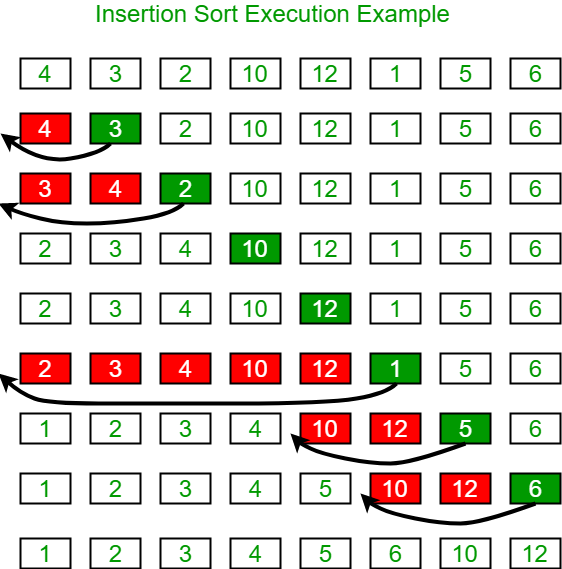
\includegraphics[scale=0.4]{insertionsort.png}}
\end{figure}

\begin{figure}[h]
\center{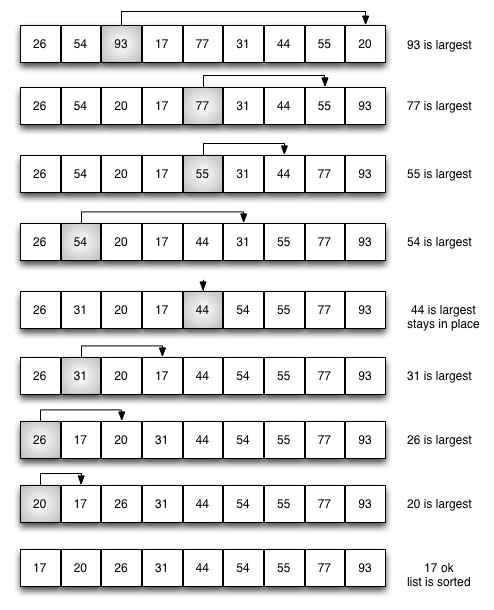
\includegraphics[scale=0.4]{selectionsortnew.png}}
\end{figure}

\textit{Мораль: нужно знать не только синтаксис, но и алгоритмы.}

\subsection{Основы программирования, основанного на событиях.}

Например, программирование систем реального времени. (+ сюда нужно добавить информацию о событийно-ориентированном программировании из конспекта Литвинова, далее речь идет про СРВ).

СРВ --- Аппаратно-программный комплекс, реагирующий за предсказуемое время на непредсказуемый поток внешних событий. То есть, события, на которые нужно реагировать, возникают в неопределенный момент времени.

Система должна успевать реагировать на одновременно происходящие события. Даже если два или больше внешних события происходят одновременно, система должна успеть среагировать на каждое из них в течение интервалов времени, критического для этих событий. То есть, события являются действиями, которые должны обрабатываться "без жужжания"{}. \textit{Возможно, Андрей Николаевич имел в виду} Джиттер (англ. jitter) — разброс значений времени отклика. Можно различить джиттер запуска (англ. release jitter) — период времени от готовности к исполнению до начала собственно исполнения задачи и джиттер вывода (англ. output jitter) — задержка по окончании выполнения задачи. Джиттер может возникать под влиянием других одновременно исполняемых задач. \textit{Но это не точно.}\\

\textbf{Процессы (задачи) систем реального времени могут иметь следующие характеристики и связанные с ними ограничения:}
\begin{enumerate}
    \item Дедлайн (англ. deadline) — критический срок обслуживания, предельный срок завершения какой-либо работы.
    \item Латентность (англ. latency) — время отклика (время задержки) системы на внешние события.
    \item Джиттер (англ. jitter) — разброс значений времени отклика.
\end{enumerate}

В зависимости от допустимых нарушений временных ограничений системы реального времени можно поделить на системы жёсткого реального времени (англ. hard real-time), для которых нарушения равнозначны отказу системы, и системы мягкого реального времени (англ. soft real-time), нарушения характеристик которых приводят лишь к снижению качества работы системы. 

Такие системы трудно отлаживать (отладчик может вносить серьезные сбои в нормальную работу системы в связи с устанавливаемыми временными ограничениями).

При создании систем реального времени приходится решать проблемы привязки внутрисистемных событий к моментам времени, своевременного захвата и освобождения системных ресурсов, синхронизации вычислительных процессов, буферизации потоков данных и т. п.\\

\textbf{Эдсгер Вибе Дейкстра --- семафоры, 1965.} Семафор --- это защищенная переменная, значение которой можно опрашивать и менять только при помощи специальных операций: P и V. Операция P блокирует семафор, операция V — деблокирует семафор. Более точно, операции P и V определены следующим образом: Операция P проверяет, что семафор открыт. Если семафор открыт, операция закрывает семафор и завершается. Операция проверки и открытия является атомарной, то есть ни один другой процесс не может наблюдать ситуации, когда семафор проверен, но ещё не закрыт. Если на момент проверки семафор уже закрыт, операция P приостановит процесс до тех пор, пока некоторый другой процесс не откроет семафор. После того, как некоторый процесс открыл семафор, система выбирает из множества процессов, ожидающих открытия семафора, какой-то один и разблокирует его. Операция V разблокирует семафор. Эта операция никогда не приостанавливает выполнение процесса. 

Семафоры со счетчиками могут принимать неотрицательные целые значения. Они используются, если некоторые ресурс выделяется из множества идентичных ресурсов. При инициализации такого семафора в его счетчике указывается число элементов множества. Каждая операция wait(s) \textit{(down)} уменьшает значения счетчика семафора s на 1, показывая, что некоторому процессу выделен один ресурс из множества. Каждая операция signal(s) \textit{(up)} увеличивает значение счетчика на 1, показывая, что процесс возвратил ресурс во множество. Если операция wait(s) выполняется, когда в счетчике содержится нуль (больше нет ресурсов), то соответствующий процесс ожидает, пока во множество не будет возвращен освободившийся ресурс, то есть пока не будет выполнена операция signal. 

\subsection{Введение в компьютерную графику: использование простых графических API.}

По способу формирования изображения различают векторные и растровые дисплеи. В векторном дисплее изображение разбивается на отдельные линии и адресация осуществляется заданием координат конечных точек каждой линии. Отрезки окружности задаются центром и радиусом или координатами трех точек. В растровых дисплеях все поле экрана представляет собой сетку, каждый узел которой есть элемент изображения (пиксел). Электронный луч пробегает все поле строка за строкой, и изменение его интенсивности вплоть до полного гашения позволяет построить полную картину с тенями и полутенями. 

Монохромные изображения кодируются с помощью одномерной шкалы яркости. Обычно это набор из чёрного и белого цвета и промежуточных оттенков серого, но могут использоваться и другие комбинации: например, монохромные мониторы часто используют зелёный или оранжевый цвет свечения вместо белого.\\

\textbf{Цветовая модель RGB.}

Эта модель описывает излучаемые цвета. Она основана на трех основных (базовых) цветах с длинами волн: 700,0 нм — красный (Red), 546,1 нм -зеленый (Green) и 435,8 нм — синий (Blue). Остальные цвета получаются сочетанием базовых. Цвета такого смешанного типа называются аддитивными. Выбор основных цветов обусловлен особенностями физиологии восприятия цвета сетчаткой человеческого глаза. Цветовая модель RGB нашла широкое применение в технике.

В компьютерах каждая из координат представляется в виде одного октета, значения которого обозначаются для удобства целыми числами от 0 до 255 включительно, где 0 — минимальная, а 255 — максимальная интенсивность. 

Цвет представляется с использованием 256 уровней для каждой из трёх компонент модели RGB: красного(R), зелёного(G) и синего(B), что в результате даёт 16 777 216 (224) различных цветов.

Обычно при кодировании пикселя на каждый из каналов (красный, зелёный, синий каналы) отводится по одному байту; четвёртый байт (если используется) обычно отводится либо для хранения данных альфа-канала, либо просто игнорируется.

\subsection{Обзор языков программирования: история языков программирования; краткий обзор парадигм программирования.}

\textbf{История языков программирования:}

\begin{itemize}
    \item На начальной стадии развития ЭВМ человеку было необходимо составлять программы на языке, понятном компьютеру, в машинных кодах. Каждая команда состояла из кода операций и адресов операндов, выраженных в виде различных сочетаний единиц и нулей.
    \item Потом для записи программ начали применять мнемонический язык — язык ассемблера. Язык ассемблера позволил представить машинный код в более удобной для человека форме: для обозначения команд и объектов, над которыми эти команды выполняются, вместо двоичных кодов использовались буквы или сокращенные слова, которые отражали суть команды.
    \item \textbf{1957} --- Fortran, Джон Бэкус, корпорация IBM, США. Первый язык программирования высокого уровня, получивший практическое применение, имеющий транслятор и испытавший дальнейшее развитие.
    \item \textbf{1958} --- Algol-58, конференция в Цюрихе, Швейцария.
    \item \textbf{1960} --- Algol-60, доработка Algol-58 на конференции в Париже. Язык обладал массой недостатков, как технических (например, использование целых числе в качестве меток) так и, собственно, языковых (например, никак не был стандартизован ввод/вывод, не была поддержана обработка литер и строк, а это уже в то время было довольно важной частью программирования, не было сложных структур данных). Поэтому авторы языка продолжили работу и в \textbf{1964} году выпустили Пересмотренное сообщение. Чтобы организационно оформить эти работы, международная федерация IFIP (International Federation for Information Processing) в 1962 г. создала Рабочую группу Working Group 2.1 по алголоподобным языкам. После выпуска Пересмотренного сообщения об Алголе 60 эта группа приступила к разработке планов следующих языков программирования – наследников Алгола 60. Была выпущена так называемая Белая книга, которая содержала несколько очень интересных статей. Например, статья Ральфа Лондона, одного из создателей языка Alphard – в котором были некоторые предпосылки для доказательств корректности программ. В статье Барбары Лисков «Язык CLU» впервые были сформулировано понятие абстрактных типов данных. Была статья голландского ученого ван Вейнгаардена о двухуровневых грамматиках.
    \item \textbf{1963} --- первый транслятор с Algol в СССР --- Лавров.
    \item \textbf{1964} --- PL/1, США. Разработан в IBM как часть системы System/360. 
    \item На основе Белой книги, а именно, на основе предложения ван Вейнгаардена, было предложено создавать новый язык, существенно более точный, с более формализованным описанием не только синтаксиса, но и семантики. В результате, после многолетних дискуссий Рабочей группы (РГ) 2.1, в работе которой приняли участие множество известных ученых из Америки и Европы, в декабре \textbf{1968} года IFIP приняла сообщение о языке Алгол 68.
    \item Язык в ту пору был очень тяжелым и трудным в понимании, поэтому РГ 2.1 продолжила свою работу, расширила состав авторов языка, и к \textbf{1973} году было подготовлено Пересмотренное сообщение об Алголе 68, в котором на основе всех базовых идей исходного языка и грамматик ван Вейнгаардена был определен существенно более приемлемый язык, более простой в реализации.
    \item \textbf{1980} --- Ada. Разработка языка была проведена в рамках международного конкурса, организованного и профинансированного министерством обороны США. Целью разработки было получение языка программирования, который мог бы стать единым для разработки проектов по заказам военного ведомства. Конкурс на его создание был объявлен в 1977 году, разработчикам было предложено базироваться на одном из трёх языков: Паскаль, Алгол-68 или ПЛ/1. Из представленных на конкурс 15 проектов было отобрано 4 (все основаны на Паскале). Эти проекты были отправлены на дальнейшую доработку. На следующем этапе из 4 проектов отобрали два, из которых, после очередной доработки, был выбран один. Этот язык получил наименование «Ада» — разработавшая его группа под руководством француза Жана Ишбиа дала языку название в честь Августы Ады Кинг Лавлейс.
    \item \textbf{1972} --- C, Bell Labs, Деннис Ритчи, Кен Томпсон. Первоначально был разработан для реализации операционной системы UNIX. Использовался, но только в 1978 появилась первая публикация по нему.
    \item \textbf{1983} --- C++, Бьёрн Страуструп. По словам Андрея Николаевича, он медленнее, чем Си, за счет загрузки объектов, в Си вложенные структуры же обрабатываются во время компиляции.
\end{itemize}

DSL (Domain Specific Language) --- Предметно-ориентированный язык, язык программирования, специализированный для конкретной области применения. У Терехова в Алголе-68 была возможность описывать свои операции, поэтому появились свои "языки"{} для бухгалтеров, для оптических вычислений и т. д.\\

\textbf{Парадигмы программирования:}

\begin{itemize}
    \item Процедурное --- создание подпрограмм, Любая программа может быть представлена как комбинация последовательно исполняемых операторов,  ветвлений и итераций.
    \item Логическое --- программа представляет собой набор фактов и правил, система сама строит решение с использованием правил логики. Создавалось в 60-х для решения задач искусственного интеллекта и экспертных систем, автоматического доказательства теорем. \textit{Если} есть конструктивное доказательство разрешимости задачи, то можем автоматически получить программу, но только \textit{если}. На практике оказалось не очень применимо.
    \item Декларативное --- говорим, что хотим получить, не говорим как. Например, язык БД SQL.
    \item Функциональное --- F\#, Haskell. Вычисления рассматриваются как вычисления значения функций в математическом понимании. Нет переменных, циклов и т.д. \textit{Андрей Николаевич не любит "функциональщину"{}.}
    \item ООП --- смотри билет один, ага.
\end{itemize}

\subsection{Виртуальные машины: понятие виртуальной машины; иерархия виртуальных машин; промежуточные языки.}

\epigraph{"Виртуальное"{} --- то чего нет, но могло бы быть. Не как бог.}{Андрей Николаевич}

Виртуальная машина - программная или аппаратная среда, эмулирующая аппаратное обеспечение некоторой платформы, исполняющая некоторый код (например, байт-код, шитый код, p-код или машинный код реального процессора), или спецификация такой системы (например: "виртуальная машина языка программирования Си"{}).\\

Изобретатель виртуальной машины --- Никлаус Вирт. В 1970 году перед ним встала задача сделать компилятор с Паскаля для множества различных компьютеров в Стенфорде. Тогда Никлаус придумал промежуточный язык P-Code, сделал компилятор с Паскаля на него на Паскале, а потом скормил ему его же собственный текст, в итоге получив компилятор с Паскаля на P-Code на языке P-Code. Последовательность p-кодов, исполнялась p-системой (интерпретатором p-кода, написанном, например, на ассемблере). Для переноса языка на новую платформу требовалось лишь адаптировать к ней p-систему, что в короткие сроки было выполнено для платформ 6502, 8080, Z-80, PDP-11 и многих других.\\

У программы может быть много уровней исполнения:

\textbf{язык высокого уровня} \Longrightarrow{} \textbf{язык ассемблера} \Longrightarrow{} \textbf{машинный код} \Longrightarrow{} \textbf{микрокоманды процессора}\\

И каждый из этих уровней можно назвать виртуальной машиной со своим промежуточным языком. 

\subsection{Введение в теорию трансляции: сравнение интерпретаторов и компиляторов; стадии трансляции; машинно-зависимая и машинно-независимая части транслятора.}

Создние трансляторов --- основа системного программирования. Транслятор (компилятор) переводит программу на некотором языке в машинные коды.\\

\textbf{Стадии трансляции:}

\begin{enumerate}
    \item \textbf{Сканер (лексический анализатор).} Выделение из литер (например в UTF-8) специальных лексем.
    \item \textbf{Парсер (синтаксический анализатор).} По лексемам строится синтаксическое дерево разбора.
    \item \textbf{Видозависимый анализ.} Получаем то же самое дерево, но типизированное, осуществляется проверка совместимости типов.
    \item \textbf{Оптимизация.} Бывает машинно-зависимая и машинно-независимая. Машинно-зависимая преобразовывает программу на уровне элементарных команд, например, инструкций процессора конкретной архитектуры. Машинно-независимая осуществляется на уровне структурных элементов программы, таких как модули, функции, ветвления, циклы.\\
    Самые часто используемые конструкции, а именно: вырезка массива, цикл и вызов процедуры особенно требуют оптимизации. 
    \item \textbf{Кодогенерация.} Машинно-зависимая часть транслятора. Конвертирует синтаксически корректную программу в последовательность инструкций, которые могут выполняться на машине.
    \item \textbf{Компоновка (линковка).} Сборка модуля из нескольких.
\end{enumerate}

Интерпретатор выполняет пооператорный (покомандный, построчный) анализ, обработку и тут же выполнение исходной программы или запроса (в отличие от компиляции, при которой программа транслируется без её выполнения). Может переводить код в промежуточное представление, полученный промежуточный код выполняется виртуальной машиной.

Во время отладки программа много раз компилируется, и поэтому для этих целей используется специальный отладочный компилятор, который работает быстрее, чем оптимизирующий.

\subsection{Введение в СУБД: история и причины возникновения систем баз данных, использование языков запросов базы данных.}

Причина возникновения: решали много задач, накопили много данных, хотим эти данные снова использовать для решения новых задач.\\

\textbf{История БД:}

\begin{itemize}
    \item \textbf{Сетевая модель} была одним из первых подходов, использовавшимся при создании баз данных в конце 50-х — начале 60-х годов. Активным пропагандистом этой модели был Чарльз Бахман. Идеи Бахмана послужили основой для разработки стандартной сетевой модели под эгидой организации CODASYL. После публикации отчетов рабочей группы этой организации многие компании привели свои сетевые базы данных более-менее в соответствие со стандартами CODASYL. 
    \item До середины 70-х годов главным конкурентом сетевых баз данных была \textbf{иерархическая модель данных}, представленная ведущим продуктом компании IBM в области баз данных — IBM IMS. Разница между иерархической моделью данных и сетевой состоит в том, что в иерархических структурах запись-потомок должна иметь в точности одного предка, а в сетевой структуре данных у потомка может иметься любое число предков. То есть иерархическая модель представляет собой связный неориентированный граф древовидной структуры, объединяющий сегменты. Иерархическая БД состоит из упорядоченного набора деревьев. Например, отечественная система ИНЕС.\\
    
    Первые БД были больше ориентированы на работу с отдельными элементами.
    
    \item В конце 60-х годов Эдгаром Коддом была предложена \textbf{реляционная модель} данных и после долгих и упорных споров с Бахманом реляционная модель приобрела большую популярность и теперь является доминирующей на рынке СУБД.
    Основаны на реляционной алгебре, состоят из таблиц. Каждая таблица состоит из столбцов (их называют полями или атрибутами) и строк (их называют записями или кортежами). Таблицы в реляционных базах данных обладают рядом свойств. Основными являются следующие:
    
    \begin{itemize}
        \item В таблице не может быть двух одинаковых строк. В математике таблицы, обладающие таким свойством, называют отношениями - по-английски relation, отсюда и название - реляционные.
        \item Столбцы располагаются в определенном порядке, который создается при создании таблицы. В таблице может не быть ни одной строки, но обязательно должен быть хотя бы один столбец.
        \item У каждого столбца есть уникальное имя (в пределах таблицы), и все значения в одном столбце имеют один тип (число, текст, дата...).
        \item На пересечении каждого столбца и строки может находиться только атомарное значение (одно значение, не состоящее из группы значений). Таблицы, удовлетворяющие этому условию, называют нормализованными.
    \end{itemize}
    
    В реляционной базе данных каждая таблица должна иметь первичный ключ — поле или комбинацию полей, которые единственным образом идентифицируют каждую строку таблицы. Если ключ состоит из нескольких полей, он называется составным. Ключ должен быть уникальным и однозначно определять запись. По значению ключа можно отыскать единственную запись. Ключи служат также для упорядочивания информации в БД.

\end{itemize}

    \textbf{Транзакция} --- неделимое действие с базой данных (нужна для защиты от сбоев).\\
    
    \textbf{СУБД} --- инструмент для работы с БД.\\
    
    Самые широко используемые СУБД: Oracle, MySQL, Microsoft SQL Server.\\
    
    \textbf{SQL} (англ. structured query language — "язык структурированных запросов"{}) — декларативный язык программирования, применяемый для создания, модификации и управления данными в реляционной базе данных. \\
    Некоторые запросы:
    \begin{verbatim}
            SELECT name, weapon FROM characters
            
            SELECT * 
            FROM characters
            WHERE weapon = 'pistol';
            
            SELECT * FROM albums WHERE genre IN ('pop','soul');
    \end{verbatim}
    
    Сегодня оптимизаторы позволяют делать множественные выборки из БД очень эффективно.\\
    
    Оперативной памяти стало больше, и многие БД размещают прямо в ней, и это быстро работает. \textit{(В интернетах пишут, что это не совсем NoSQL, как говорил Терехов, а "Резидентная база данных"{} (англ. in-memory database, IMDB))}

\subsection{Эволюция программ: сопровождение программ, характеристики удобного для сопровождения программного обеспечения, реинжиниринг, унаследованные системы, повторное использование программного обеспечения.}

\epigraph{Надо так давать, чтобы можно было взять.}{В. Осеева, "Синие листья"{}, сказка}

\textit{maintenance} \sim{} \textit{evolution}\\

Только 30\% бюджета уходит на разработку программного продукта, остальное --- на сопровождение.
Сопровождение включает в себя доработку, исправление, оптимизацию ПО.\\

\textbf{Характеристики удобного для сопровождения ПО:}

\begin{itemize}
    \item readability
    \item хорошая система сообщения об ошибках
    \item хорошая система тестирования
    \item документация
\end{itemize}

\textbf{Средства сопровождения ПО:}

\begin{itemize}
    \item \textbf{Профилятор.} Собирает характеристики работы программы. Принцип Парето --- 95\% времени исполнения программы приходятся на 5\% текста. (в оригинале --- "20\% усилий дают 80\% результата, а остальные 80\% усилий — лишь 20\% результата"{}).
    \item \textbf{Анализатор.}  Статический (без реального выполнения исследуемых программ) и динамический анализ программного обеспечения.
\end{itemize}

\textbf{Трехмерное проектирование} --- 3D зависимость между поведением, функциональностью и структурой программы, должна быть проекция на каждую из этих осей.\\

\textbf{Legacy code} --- устаревший код, который более не поддерживается и не обновляется, но используется.\\

\begin{figure}[h]
\center{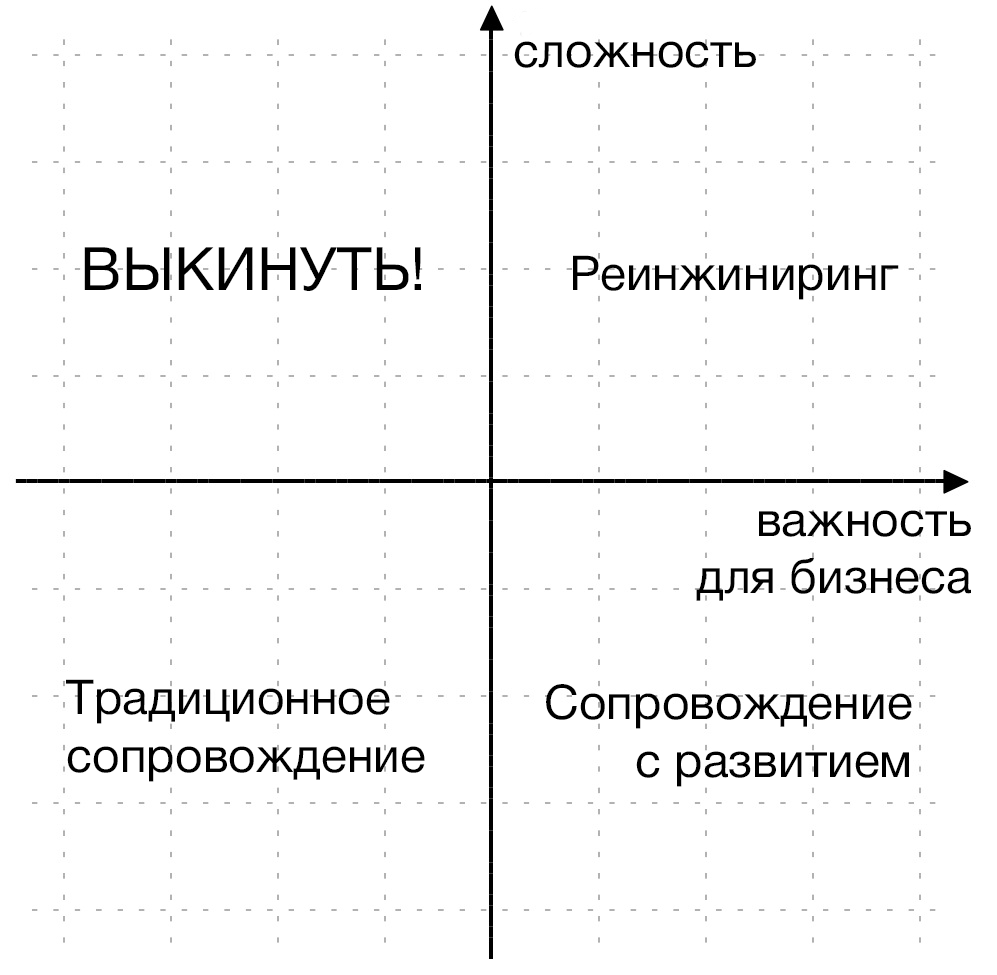
\includegraphics[scale=0.25]{graph.png}}
\end{figure}

\textbf{Терехов про "Rescue Ware"{}:}

<<Примерно в конце 1992 года через одного бывшего ленинградца (а в то время уже
американца) мне в руки попало письмо от американской компании Seer Technologies с
приглашением принять участие в проекте по реинжинирингу устаревших программных
систем. На самом деле, это письмо не было адресовано мне или нашей компании, они уже
сделали несколько попыток как в США, так и в России. Американская бизнес-идея
выглядела очень привлекательной: в мире накоплены тонны программ, написанных на
Cobol, PL/1, Adabas Natural и других устаревших языках. Эти программы успешно
эксплуатируются более 10-20 лет, причем в критически важных областях (оборона,
финансы, здравоохранение и т.п.), но их сопровождение с каждым годом становится всё
дороже. Авторы программ уже не работают в данной фирме, университеты не готовят
специалистов по старым языкам, никто не поддерживает технологии, с помощью которых
это ПО было реализовано. Самое страшное, из-за многочисленных изменений, сделанных 
в ПО за долгие годы эксплуатации, документация не отражает реальное положение дел.
Таким образом, единственным источником реальной информации о программе является её
исходный код (текст программы). А поскольку американцы всегда славились своей
приверженностью к методу «грубой силы», то приложение объемом 4-5 млн строк,
состоящее из модулей по 40-60 тыс.строк на 10-15 разных языках, не является редкостью.
С другой стороны, даже понимание логики работы программы, а, тем более,
перевод её на современные платформы, требуют глубокого и детального её анализа (граф
потоков данных, граф потоков управления, граф окон взаимодействия с человеком, базами
данных и т.д.), а, как известно, числе путей в графе растет экспоненциально относительно
числа узлов в этом графе, т.е. анализ, написанный «в лоб», будет работать очень долго.
В решении этой задачи нам очень помог наш многолетний опыт создания
трансляторов и сильная математическая подготовка наших сотрудников. Реинжиниринг
дам нал массу совершенно новых задач, по которым было защищено несколько десятков
дипломных работ, защищено три кандидатские диссертации [Терехов мл., Эрлих,
Мосиенко].
Получившийся в результате продукт Rescue Ware в 2000 и 2001 годах Gartner Group
признавала лучшим в области Legacy Understanding и Legacy Transformation. Был период,
когда над этим продуктом у нас работало более 100 человек. Мы получили неоценимый
опыт разработки программного продукта (а не традиционного для нас сервисного
программирования на заказ), настоящей промышленной разработки с выходом на
американский рынок.>>

\section{CS103. Алгоритмы и структуры данных.}

\subsection{Базовые структуры данных: стеки, очереди, связанные списки, хэш-таблицы, деревья, графы.}

\textbf{Стеки и очереди} — это динамические множества, элементы из которых удаляются с помощью предварительно определенной операции DELETE. Первым из стека (stack) удаляется элемент, который был помещен туда последним: в стеке реализуется стратегия “последним вошел — первым вышел” (last-in, first-out — LIFO).

Аналогично, в очереди (queue) всегда удаляется элемент, который содержится
в множестве дольше других: в очереди реализуется стратегия “первым вошел —
первым вышел” (first-in, first-out — FIFO). Существует несколько эффективных
способов реализации стеков и очередей в компьютере. 

Операция вставки применительно к стекам часто называется PUSH (запись
в стек), а операция удаления — POP (снятие со стека).

Применительно к очередям операция вставки называется ENQUEUE (поместить
в очередь), а операция удаления — DEQUEUE (вывести из очереди). Подобно стековой операции POP, операция DEQUEUE не требует передачи элемента массива
в виде аргумента. Благодаря свойству FIFO очередь подобна, например, живой
очереди к врачу в поликлинике. У нее имеется голова (head) и хвост (tail). Когда
элемент ставится в очередь, он занимает место в ее хвосте, точно так же, как
человек занимает очередь последним, чтобы попасть на прием к врачу. Из очереди всегда выводится элемент, который находится в ее головной части аналогично
тому, как в кабинет врача всегда заходит больной, который ждал дольше всех.\\

\textbf{Связанный список (linked list)} — это структура данных, в которой объекты
расположены в линейном порядке. Однако, в отличие от массива, в котором этот
порядок определяется индексами, порядок в связанном списке определяется указателями на каждый объект. Связанные списки обеспечивают простое и гибкое
представление динамических множеств.

Списки могут быть разных видов. Список может быть однократно или дважды
связанным, отсортированным или неотсортированным, кольцевым или некольцевым. Если список однократно связанный (однонаправленный) (singly linked), то
указатель prev в его элементах отсутствует. Если список отсортирован (sorted),
то его линейный порядок соответствует линейному порядку его ключей; в этом
случае минимальный элемент находится в голове списка, а максимальный — в его
хвосте. Если же список не отсортирован, то его элементы могут располагаться в произвольном порядке. Если список кольцевой (circular list), то указатель prev его головного элемента указывает на его хвост, а указатель next хвостового
элемента — на головной элемент. Такой список можно рассматривать как замкнутый в виде кольца набор элементов.\\

\textbf{Хеш-таблица} представляет собой эффективную структуру данных для реализации словарей. Хотя на поиск элемента
в хеш-таблице может в наихудшем случае потребоваться столько же времени, что
и в связанном списке, а именно O(n), на практике хеширование исключительно
эффективно.

В случае прямой адресации элемент с ключом k хранится в ячейке k. При
хешировании этот элемент хранится в ячейке h(k), т.е. мы используем хеш-функцию h для вычисления ячейки для данного ключа k. Функция h отображает пространство ключей на ячейки хеш-таблицы.\\

\textbf{Дерево} — это связный ациклический граф. Связность означает наличие путей между любой парой вершин, ацикличность — отсутствие циклов и то, что между парами вершин имеется только по одному пути.

Путём из n1 в nk называют последовательность узлов n1, ..., nk, в котором каждый узел является родителем следующего. Длина пути — число, на единицу меньшее количества узлов, составляющих путь.
Путь нулевой длины — путь из узла к самому себе.
Узел a называется предком узла b, если существует путь из a в b. b в этом случае — потомок a. Каждый узел — предок и потомок самого себя. Потомок, не являющийся самим узлом, называется истинным потомком, с предком аналогично.
Узел, не имеющий истинных потомков, называется листом.
Поддерево какого-либо дерева — узел вместе со всеми потомками.
Высота узла — длина самого длинного пути из узла до какого-либо листа, глубина узла — длина пути от узла до корня. Высота дерева — высота корня.

Деревья бывают упорядоченными и неупорядоченными. Можно упорядочить узлы дерева, не связанные отношением предок-потомок (слева-справа).

\textbf{Обходы дерева}
\begin{itemize}
    \item Прямой порядок — сначала корень, потом сыновья по порядку.
    \item Симметричный порядок — сначала первый сын, затем корень, затем остальные сыновья.
    \item Обратный порядок — сначала сыновья, потом корень.
\end{itemize}

Двоичные деревья — это деревья, в которых у каждого узла есть левый и правый сын, причём это принципиально разные вещи.

Двоичное дерево поиска — дерево, узлы которого помечены элементами множества, над которым определено отношение полного порядка.
Определяющее свойство BST — все элементы, хранящиеся в узлах левого поддерева любого узла x, меньше элемента, содержащегося в x, а в узлах правого поддерева — больше.
Если обойти двоичное дерево в симметричном порядке, получится список элементов, упорядоченный по возрастанию.\\

\textbf{Граф} — абстрактный математический объект, представляющий собой множество вершин графа и набор рёбер, то есть соединений между парами вершин.

Графы бывают ориентированные и неориентированные. 
Ориентированный граф (орграф) G — это пара из множества вершин V и множества дуг E, где E — упорядоченная пара вершин (v, w) (т.е. E — бинарное отношение над множеством вершин). v называется началом, w — концом дуги. Рёбра вида (v, v) называются петлями.
Путём в орграфе называется последовательность вершин, для которых существуют дуги из предыдущей в следующую. Длина пути — количество дуг, составляющих путь. Путь называется простым, если все вершины на нём, за исключением, быть может, первой и последней, различны. Цикл — это простой путь длины не менее 1, который начинается и заканчивается в одной вершине. Если в графе нет циклов, он называется ациклическим. Граф может быть помеченным.
Неориентированный граф — это ориентированный граф, у которого для каждого ребра (v, w) существует противоположное ребро (w, v), то есть отношение E симметрично. Если e = (u,v) принадлежит E, то вершины u и v называются смежными в G, а ребро e и эти вершины называются инцидентными. Степенью вершины в неориентированном графе называется число смежных с ней вершин. Вершина степени 0 называется изолированной.


\subsection{Основные вычислительные алгоритмы: алгоритмы сортировки со сложностью O(NlogN), хэш-таблицы и алгоритмы избежания коллизий.}

\textbf{Сортировка слиянием}, или сортировка фон Неймана (англ. merge sort) — алгоритм сортировки, который упорядочивает списки (или другие структуры данных, доступ к элементам которых можно получать только последовательно, например — потоки) в определённом порядке. Эта сортировка — хороший пример использования принципа «разделяй и властвуй». Сначала задача разбивается на несколько подзадач меньшего размера. Затем эти задачи решаются с помощью рекурсивного вызова или непосредственно, если их размер достаточно мал. Наконец, их решения комбинируются, и получается решение исходной задачи.

Алгоритм был изобретён Джоном фон Нейманом в 1945 году.\\

Сортируемый массив разбивается на две части примерно одинакового размера;
Каждая из получившихся частей сортируется отдельно, например — тем же самым алгоритмом;
Два упорядоченных массива половинного размера соединяются в один.\\

\textbf{Стадии: }

\begin{enumerate}
    \item Рекурсивное разбиение задачи на меньшие происходит до тех пор, пока размер массива не достигнет единицы (любой массив длины 1 можно считать упорядоченным).
    \item Соединение двух упорядоченных массивов в один.
    Основную идею слияния двух отсортированных массивов можно объяснить на следующем примере. Пусть мы имеем два уже отсортированных по возрастанию подмассива. Тогда:
    \begin{enumerate}
        \item Слияние двух подмассивов в третий результирующий массив.
    На каждом шаге мы берём меньший из двух первых элементов подмассивов и записываем его в результирующий массив. Счётчики номеров элементов результирующего массива и подмассива, из которого был взят элемент, увеличиваем на 1.
        \item «Прицепление» остатка. Когда один из подмассивов закончился, мы добавляем все оставшиеся элементы второго подмассива в результирующий массив.
    \end{enumerate}
\end{enumerate}

\textbf{Достоинства: }

\begin{itemize}
    \item Не имеет «трудных» входных данных.
    \item Устойчивая - сохраняет порядок равных элементов (принадлежащих одному классу эквивалентности по сравнению).
    \item Внешняя (подходит для больших данных, не помещающихся в память).
\end{itemize}

\textbf{Недостатки: }

\begin{itemize}
    \item На «почти отсортированных» массивах работает столь же долго, как на хаотичных.
    \item Требует дополнительной памяти по размеру исходного массива.
\end{itemize}

\textbf{Пирамидальная сортировка} (англ. Heapsort, «Сортировка кучей») — алгоритм сортировки, работающий в худшем, в среднем и в лучшем случае (то есть гарантированно) за O(n log n) операций при сортировке n элементов. Количество применяемой служебной памяти не зависит от размера массива (то есть, O(1)).\\

Сортировка пирамидой использует бинарное сортирующее дерево. Сортирующее дерево (двоичная куча) — это такое дерево, у которого выполнены условия:

\begin{enumerate}
    \item Значение в любой вершине не меньше, чем значения её потомков.
    \item Глубина всех листьев (расстояние до корня) отличается не более чем на 1 слой.
    \item Последний слой заполняется слева направо без «дырок».
\end{enumerate}

Удобная структура данных для сортирующего дерева — такой массив Array, что Array[0] — элемент в корне, а потомки элемента Array[i] являются Array[2i+1] и Array[2i+2].\\

Необходимо отсортировать массив A, размером n. Построим на базе этого массива за O(n) кучу для максимума. Так как максимальный элемент находится в корне, то если поменять его местами с A[n−1], он встанет на своё место. Далее вызовем процедуру siftDown(0), предварительно уменьшив heapSize на 1. Она за ${\displaystyle O(\log n)}$ просеет A[0] на нужное место и сформирует новую кучу (так как мы уменьшили её размер, то куча располагается с A[0] по A[n−2], а элемент A[n−1] находится на своём месте). Повторим эту процедуру для новой кучи, только корень будет менять местами не с A[n−1], а с A[n−2]. Делая аналогичные действия, пока heapSize не станет равен 1, мы будем ставить наибольшее из оставшихся чисел в конец не отсортированной части.\\

\textbf{Достоинства: }

\begin{itemize}
    \itemИмеет доказанную оценку худшего случая ${\displaystyle O(n\cdot \log n)}$.
    \item Сортирует на месте, то есть требует всего O(1) дополнительной памяти.
\end{itemize}

\textbf{Недостатки: }

\begin{itemize}
    \item Требует произвольного доступа к памяти.
    \item Неустойчива.
\end{itemize}

\textbf{Быстрая сортировка}, сортировка Хоара (англ. quicksort), — алгоритм сортировки, разработанный английским информатиком Чарльзом Хоаром во время его работы в МГУ в 1960 году.\\

Общая идея алгоритма состоит в следующем:

\begin{itemize}
    \item Выбрать из массива элемент, называемый опорным. Это может быть любой из элементов массива. От выбора опорного элемента не зависит корректность алгоритма, но в отдельных случаях может сильно зависеть его эффективность.
    \item Сравнить все остальные элементы с опорным и переставить их в массиве так, чтобы разбить массив на три непрерывных отрезка, следующих друг за другом: «элементы меньшие опорного», «равные» и «большие». 
    \item Для отрезков «меньших» и «больших» значений выполнить рекурсивно ту же последовательность операций, если длина отрезка больше единицы.
\end{itemize}

\textbf{Недостатки: }

\begin{itemize}
    \item Сильно деградирует по скорости (до ${\displaystyle O(n^{2})}$) в худшем или близком к нему случае, что может случиться при неудачных входных данных.
    \item Неустойчива.
\end{itemize}

\textbf{Алгоритмы избежания коллизий: }\\

\textbf{Метод цепочек.} Каждая ячейка массива H является указателем на связный список (цепочку) пар ключ-значение, соответствующих одному и тому же хеш-значению ключа. Коллизии просто приводят к тому, что появляются цепочки длиной более одного элемента.
Операции поиска или удаления элемента требуют просмотра всех элементов соответствующей ему цепочки, чтобы найти в ней элемент с заданным ключом. Для добавления элемента нужно добавить элемент в конец или начало соответствующего списка, и в случае, если коэффициент заполнения станет слишком велик, увеличить размер массива H и перестроить таблицу.

\textbf{Открытая адресация.} В массиве H хранятся сами пары ключ-значение. Алгоритм вставки элемента проверяет ячейки массива H в некотором порядке до тех пор, пока не будет найдена первая свободная ячейка, в которую и будет записан новый элемент. Этот порядок вычисляется на лету, что позволяет сэкономить на памяти для указателей, требующихся в хеш-таблицах с цепочками. Последовательность, в которой просматриваются ячейки хеш-таблицы, называется последовательностью проб.

\begin{itemize}
    \item Линейное пробирование: ячейки хеш-таблицы последовательно просматриваются с некоторым фиксированным интервалом k между ячейками (обычно, k = 1), то есть i-й элемент последовательности проб — это ячейка с номером (hash(x) + i*k) mod N. Для того, чтобы все ячейки оказались просмотренными по одному разу, необходимо, чтобы k было взаимно-простым с размером хеш-таблицы.
    \item Квадратичное пробирование: интервал между ячейками с каждым шагом увеличивается на константу. Если размер хеш-таблицы равен степени двойки (N = 2p), то одним из примеров последовательности, при которой каждый элемент будет просмотрен по одному разу, является: hash(x) mod N, (hash(x) + 1) mod N, (hash(x) + 3) mod N, (hash(x) + 6) mod N, …
\end{itemize}

\subsection{Двоичные деревья поиска, представления графов, обходы в глубину и в ширину.}

\textbf{АВЛ-дерево} — сбалансированное по высоте двоичное дерево поиска: для каждой его вершины высота её двух поддеревьев различается не более чем на 1.

АВЛ — аббревиатура, образованная первыми буквами фамилий создателей (советских учёных) Адельсон-Вельского Георгия Максимовича и Ландиса Евгения Михайловича. (Создавалось для реализации библиотеки эндшпилей в шахматной программе "Каисса"{}).

\begin{figure}[h]
\center{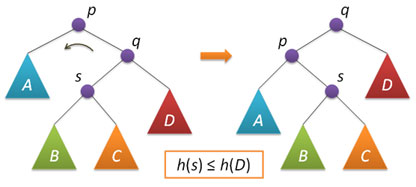
\includegraphics[scale=0.5]{avl1.jpg}}
\end{figure}

\begin{figure}[h]
\center{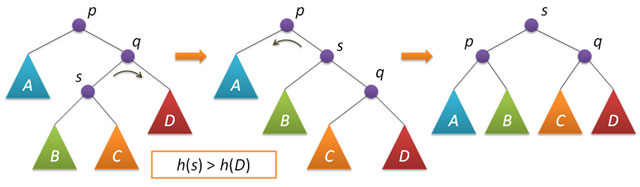
\includegraphics[scale=0.5]{avl2.jpg}}
\end{figure}

\textbf{Представления графов: }

\begin{itemize}
    \item \textbf{Матрица смежности.} Для графа из n вершин матрица смежности — матрица размера n на n, где в строке i и столбце j стоит 1 (или true), если есть дуга из i в j. Для неориентированного графа матрица симметрична относительно главной диагонали. Для взвешенного графа вместо 1 стоит вес дуги.
    \item \textbf{Матрица инцидентности.}Для графа из n вершин и mребёр матрица
инцидентности — матрица размера m на n, где строка соответствует вершине, а столбец ребру.  Для ориентированного графа в ячейке (i,j) стоит 1, если ребро i выходит из вершины j, и -1, если входит. Для неориентированного графа в ячейке (i,j) стоит 1, если ребро i инцидентно вершине j. Нужно специальное значение для петель.
    \item \textbf{Список смежности.} Для каждой вершины хранится список вершин, смежных с данной. Как правило, списки лежат в массиве длины n. Вместе с номером смежной вершины в списке может лежать вес ребра.
\end{itemize}

\subsection{Рекурсия: понятие рекурсии, рекурсивные математические функции, простые рекурсивные процедуры, стратегия «разделяй и властвуй», рекурсивный перебор с возвратами, реализация рекурсии.}

\textbf{Рекурсия} --- вызов функцией самой себя (причем не обязательно непосредственно).

Любой рекурсивный алгоритм можно переписать без использования рекурсии.

\textbf{Головная рекурсия} — рекурсивный вызов выполняется ближе к началу метода и является одним из первых обрабатываемых объектов. Поскольку он вызывает сам себя, ему приходится полагаться на результаты предыдущей операции, помещенной в стек вызовов. Из-за использования стека вызовов существует вероятность переполнения стека, если стек вызовов недостаточно велик.

\textbf{Хвостовая рекурсия} — частный случай рекурсии, при котором любой рекурсивный вызов является последней операцией перед возвратом из функции. Подобный вид рекурсии примечателен тем, что может быть легко заменён на итерацию путём формальной и гарантированно корректной перестройки кода функции. Оптимизация хвостовой рекурсии путём преобразования её в плоскую итерацию реализована во многих оптимизирующих компиляторах. В некоторых функциональных языках программирования спецификация гарантирует обязательную оптимизацию хвостовой рекурсии.

В точке вызова в стек помещаются параметры, передаваемые функции, и адрес возврата.
Вызываемая функция в ходе работы размещает в стеке собственные локальные переменные.
По завершении вычислений функция очищает стек от своих локальных переменных, записывает результат (обычно — в один из регистров процессора). Команда возврата из функции считывает из стека адрес возврата и выполняет переход по этому адресу. Либо непосредственно перед, либо сразу после возврата из функции стек очищается от параметров.

Нетрудно видеть, что необходимость расширения стека при рекурсивных вызовах диктуется требованием восстановления состояния вызывающего экземпляра функции (то есть её параметров, локальных данных и адреса возврата) после возврата из рекурсивного вызова. Но если рекурсивный вызов является последней операцией перед выходом из вызывающей функции и результатом вызывающей функции должен стать результат, который вернёт рекурсивный вызов, сохранение контекста уже не имеет значения — ни параметры, ни локальные переменные уже использоваться не будут, а адрес возврата уже находится в стеке. Поэтому в такой ситуации вместо полноценного рекурсивного вызова функции можно просто заменить значения параметров в стеке и передать управление на точку входа. До тех пор, пока исполнение будет идти по этой рекурсивной ветви, будет, фактически, выполняться обычный цикл. Когда рекурсия завершится (то есть исполнение пройдёт по терминальной ветви и достигнет команды возврата из функции) возврат произойдёт сразу в исходную точку, откуда произошёл вызов рекурсивной функции. Таким образом, при любой глубине рекурсии стек переполнен не будет.

В РуСи "program counter"{} --- указатель на то место, где функция была прервана, и вызвала другую.

Реализация вызова рекурсивной функции не отличается от реализации вызова обычной функции.\\

\textbf{Примеры использования рекурсии: }

\begin{itemize}
    \item Обход дерева.
    \item Динамическое программирование. Метод решения задач путем составления последовательности из подзадач таким образом, что: первый элемент последовательности (возможно несколько элементов) имеет тривиальное решение, последний элемент этой последовательности - это исходная задача, каждая задача этой последовательности может быть решена с использованием решения подзадач с меньшими номерами. Динамическое программирование обычно придерживается двух подходов к решению задач:
    
    Нисходящее ДП: задача разбивается на подзадачи меньшего размера, они решаются и затем комбинируются для решения исходной задачи. Используется запоминание для решений часто встречающихся подзадач.
    
    Восходящее ДП: Все подзадачи, которые впоследствии понадобятся для решения исходной задачи просчитываются заранее и затем используются для построения решения исходной задачи. Этот способ лучше нисходящего ДП в смысле размера необходимого стека и количества вызова функций, но иногда бывает нелегко заранее выяснить решение каких подзадач нам потребуется в дальнейшем.
\end{itemize}

\textbf{Поиск с возвратом, бэктрекинг} (англ. backtracking) — общий метод нахождения решений задачи, в которой требуется полный перебор всех возможных вариантов в некотором множестве М. Как правило позволяет решать задачи, в которых ставятся вопросы типа: «Перечислите все возможные варианты …», «Сколько существует способов …», «Есть ли способ …», «Существует ли объект…» и т. п.

Решение задачи методом поиска с возвратом сводится к последовательному расширению частичного решения. Если на очередном шаге такое расширение провести не удается, то возвращаются к более короткому частичному решению и продолжают поиск дальше. Данный алгоритм позволяет найти все решения поставленной задачи, если они существуют. Для ускорения метода стараются вычисления организовать таким образом, чтобы как можно раньше выявлять заведомо неподходящие варианты. Зачастую это позволяет значительно уменьшить время нахождения решения.

Классическим примером использования алгоритма поиска с возвратом является задача о восьми ферзях. Её формулировка такова: «Расставить на стандартной 64-клеточной шахматной доске 8 ферзей так, чтобы ни один из них не находился под боем другого». Сперва на доску ставят одного ферзя, а потом пытаются поставить каждого следующего ферзя так, чтобы его не били уже установленные ферзи. Если на очередном шаге такую установку сделать нельзя — возвращаются на шаг назад и пытаются поставить ранее установленного ферзя на другое место.

Метод поиска с возвратом является универсальным. Достаточно легко проектировать и программировать алгоритмы решения задач с использованием этого метода. Однако время нахождения решения может быть очень велико даже при небольших размерностях задачи (количестве исходных данных), причём настолько велико (может составлять годы или даже века), что о практическом применении не может быть и речи. Поэтому при проектировании таких алгоритмов, обязательно нужно теоретически оценивать время их работы на конкретных данных.

\subsection{Базовый анализ алгоритмов: асимптотический анализ максимальной и средней сложности; установление различий между лучшим, средним и худшим случаями; нотации «О-большое» и «о-маленькое», «омега» и «тета»; стандартные классы сложности.}

O: в научных трудах O описывает верхнюю границу вычислительной сложности.
Сложность алгоритма, выводящего все значения из массива, может быть описана
обозначением O(N), но также ее можно описать обозначениями O($N^2$), O($N^3$) или
O($2^N$) (и многими другими). Алгоритм по крайней мере не превосходит их по
скорости; следовательно, все эти варианты описывают верхнюю границу сложности. Ситуацию можно сравнить с отношениями «меньше либо равно»: если Бобу
исполнилось X лет (будем считать, что предельный срок жизни равен 130 годам),
то можно утверждать, что X $≤$ 130. Также будет правильно утверждать, что X $<=$ 1000
или X $<=$ 1 000 000. Формально эти утверждения верны (хотя особой пользы и не приносят).

$\Omega{}$: в научных трудах $\Omega{}$ представляет эквивалентную концепцию для нижней границы. Сложность вывода значений из массива может быть описана обозначением $\Omega{}$(N), равно как и обозначениями $\Omega{}$(log N) и $\Omega{}$(1). Вы уверены в том, что быстрее она работать не будет.

$\Theta{}$: в научных трудах $\Theta{}$ подразумевает как O, так и $\Omega{}$. Иначе говоря, алгоритм имеет
сложность $\Theta{}$(N), если он одновременно обладает сложностью O(N) и $\Omega{}$(N). $\Theta{}$ определяет точную границу сложности.
На практике (а следовательно, и на собеседованиях) смысл $\Theta{}$ и O практически
смешался. Представления об O в среде разработчиков ближе к тому, что теоретики
подразумевают под $\Theta{}$, так что описание сложности вывода массива в виде O($N^2$)
будет воспринято как ошибочное. Вероятно, специалист-практик скажет, что эта
операция имеет сложность O(N).

\begin{figure}[h]
\center{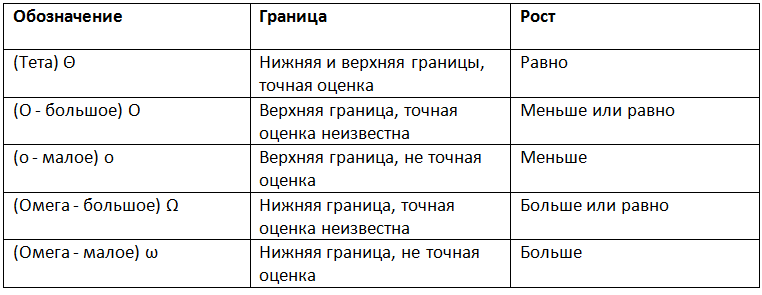
\includegraphics[scale=0.5]{notation.png}}
\end{figure}

В теории вычислительной сложности сложность алгоритма в среднем — это количество неких вычислительных ресурсов (обычно — время), требуемое для работы алгоритма, усреднённое по всем возможным входным данным. Понятие часто противопоставляется максимальной сложности, где рассматривается максимальная сложность алгоритма по всем входным данным. Имеются три основных причины изучения сложности в среднем. Во-первых, хотя некоторые задачи могут быть трудно разрешимы в худшем случае, входные данные, которые приводят к такому поведению, на практике встречаются редко, так что сложность в среднем может оказаться более аккуратной мерой производительности алгоритма. Во-вторых, анализ сложности в среднем даёт средства и технику генерации сложных данных для задачи, что можно использовать в криптографии и в-третьих, сложность в среднем позволяет выделить наиболее эффективный алгоритм на практике среди алгоритмов той же основной сложности (например, быстрая сортировка). Анализ алгоритмов в среднем требует понятия «средних» данных алгоритма, что приводит к задаче продумывания распределения вероятностей входных данных. Может быть использован также вероятностный алгоритм. Анализ таких алгоритмов приводит к связанному понятию ожидаемой сложности.\\

Лучший случай: если все элементы равны, то алгоритм быстрой сортировки
в среднем переберет массив всего один раз. Это соответствует времени O(N).
(На самом деле оценка частично зависит от реализации быстрой сортировки —
существуют реализации, которые очень быстро работают с отсортированными
массивами.)

Худший случай: а если в результате хронического невезения в качестве опорного
будет постоянно выбираться наибольший элемент массива? (Кстати, это вполне
возможно, если в качестве опорного выбирается первый элемент подмассива,
а сам массив отсортирован в обратном порядке.) Тогда рекурсия не делит массив
надвое, а всего лишь уменьшает подмассив на один элемент. В этом вырожденном
случае время выполнения достигает O(N2).

Ожидаемый случай: впрочем, обычно такие замечательные или ужасные ситуации не встречаются. Конечно, в отдельных случаях опорное значение может
оказаться очень высоким или низким, но такие аномалии не будут повторяться
снова и снова. В среднем время выполнения составит O(N log N).\\

В системах реального времени и на практике важна максимальная сложность.\\

Сложность бывает не только вычислительная, но и емкостная: сколько дополнительной памяти требует программа. Причем часто бывает так, что одна переводится в другую.\\

Те задачи, время решения которых (количество операций для нахождения ответа) зависит от количества входных данных, как многочлен, называются принадлежащими к P-классу (polynomial) алгоритмов. Те задачи, для которых можно хотя бы проверить правильность предложенного решения за полиномиально зависящее от входных данных время, называются принадлежащими NP-классу (non-deterministic polynomial). P-класс входит в NP-класс. А NP-полные задачи - те, для которых не доказано ни то, что они не могут быть решены за полиномиальное время, ни то, что они не могут быть решены за полиномиальное время (то есть они NP, но неизвестно, может, они и P, но это не доказать) . Это целый класс задач, для которого известно, что если когда-нибудь удастся доказать, что хоть одна задача из них принадлежит классу P, то все задачи этого класса будут принадлежать классу P - но еще ни для одной задачи этого класса не удалось найти полиномиальный алгоритм решения.

\subsection{Эмпирические измерения производительности; затраты по времени и объему памяти; использование рекуррентных соотношений для анализа рекурсивных алгоритмов.}

\textit{ЭМПИРИЧЕСКИЙ} --- основанный на опыте, изучении фактов, опирающийся на непосредственное наблюдение, эксперимент.\\

Empirical software engineering включает в себя замеры производительности по различным параметрам (в том числе и связанных с работой людей) и устранение "bottleneck"{}ов.\\

\textit{Регулярные оценки на длительные сроки.}\\

Эмпирические модели производительности строятся на основе анализа данных, полученных при измерении параметров рабочей нагрузки и соответствующих значений производительности системы.\\

Эмпирическая модель может быть представлена в виде таблицы или графика.\\

Если алгоритм рекуррентно вызывает сам себя, время его работы часто можно описать с помощью рекуррентного соотношения. Рекуррентное соотношение (recurrence) — это уравнение или неравенство, описывающее функцию с использованием ее самой, но только с меньшими аргументами.\\

\textbf{Основная теорема о рекуррентных соотношениях} (англ. Master theorem) используется в анализе алгоритмов для получения асимптотической оценки рекурсивных соотношений (рекуррентных уравнений), часто возникающих при анализе алгоритмов типа «разделяй и властвуй» (divide and conquer), например, при оценке времени их выполнения. 

\begin{verbatim}
    function T(input n: размер задачи):
  if n < некоторая константа k:
    решить задачу относительно n нерекурсивно
  else:
    определить множество из a подзадач, каждая размера n/b
    вызвать функцию T рекурсивно для каждой подзадачи
    объединить решения
  end
\end{verbatim}

В приведенном примере алгоритм рекурсивно разделяет исходную задачу размера n на несколько новых подзадач, каждая размером n/b. Такое разбиение может быть представлено в виде дерева вызовов, в котором каждый узел соответствует рекурсивному вызову, а ветви, исходящие из узла — последующим вызовам для подзадач. Каждый узел будет иметь a ветвей. Также в каждом узле производится объём работы, соответствующий размеру текущей подзадачи n (переданному в данный вызов функции) согласно соотношению $f(n)$. Общий объем работы алгоритма определяется как сумма всех работ в узлах данного дерева.

Вычислительная сложность подобных алгоритмов может быть представлена в виде рекуррентного соотношения

${\displaystyle T(n)=a\;T\left({\frac {n}{b}}\right)+f(n)}$. Его можно решить путём многократных подстановок выражения ${\displaystyle T\left({\frac {n}{b}}\right)}$.

С помощью основной теоремы возможно быстрое вычисление подобных соотношений, что позволяет получить асимптотическую оценку времени работы рекурсивных алгоритмов в нотации O(n) ($\Theta$-нотации), не производя подстановок.

В применении к анализу алгоритмов константы и функции обозначают:
n — размер задачи.

a — количество подзадач в рекурсии.

n/b — размер каждой подзадачи. (Предполагается, что все подзадачи на каждом этапе имеют одинаковый размер.)

f (n) — оценка сложности работы, производимой алгоритмом вне рекурсивных вызовов. В неё также включается вычислительная стоимость деления на подзадачи и объединения результатов решения подзадач.

Основная теорема позволяет получить асимптотическую оценку для следующих трех случаев:

\begin{enumerate}
    \item Если $f(n)=O\left(n^{{c}}\right)$, и выполняется соотношение $c<\log _{b}a$

тогда:

$T(n)=\Theta \left(n^{{\log _{b}a}}\right)$

    \item Если для некоторой константы k ≥ 0 выполняется:

$f(n)=\Theta \left(n^{{c}}\log ^{{k}}n\right)$ где $c=\log _{b}a$
тогда:

$T(n)=\Theta \left(n^{{c}}\log ^{{k+1}}n\right)$

    \item Если выполняется:

$f(n)=\Omega \left(n^{{c}}\right)$ где $c>\log _{b}a$
а также верно, что:

$af\left({\frac  {n}{b}}\right)\leq kf(n)$ для некоторой константы $k<1$ и достаточно больших n (так называемое условие regularity condition)
тогда:

$ T\left(n\right)=\Theta \left(f(n)\right)$

\end{enumerate}

В \textit{методе подстановок (substitution method)} нужно догадаться, какой вид имеют
граничные функции, а затем с помощью метода математической индукции доказать, что догадка правильная. В методе \textbf{деревьев рекурсии (recursion-tree method)}
рекуррентное соотношение преобразуется в дерево, узлы которого представляют
время выполнения каждого уровня рекурсии; затем для решения соотношения
используется метод оценки сумм.

\subsection{Алгоритмические стратегии: методы «грубой силы»; «жадные» алгоритмы; «разделяй и властвуй»; алгоритмы с возвратами; метод ветвей и границ.}

\textbf{Разделяй и властвуй} (англ. divide and conquer) в информатике — важная парадигма разработки алгоритмов, заключающаяся в рекурсивном разбиении решаемой задачи на две или более подзадачи того же типа, но меньшего размера, и комбинировании их решений для получения ответа к исходной задаче; разбиения выполняются до тех пор, пока все подзадачи не окажутся элементарными.

\textbf{Жадный алгоритм} — алгоритм, заключающийся в принятии локально оптимальных решений на каждом этапе, допуская, что конечное решение также окажется оптимальным. Алгоритмы Дейкстры, Краскала, Прима.

\textbf{Полный перебор} (или метод «грубой силы», англ. brute force) — метод решения математических задач. Относится к классу методов поиска решения исчерпыванием всевозможных вариантов. Сложность полного перебора зависит от количества всех возможных решений задачи. Если пространство решений очень велико, то полный перебор может не дать результатов в течение нескольких лет или даже столетий.

\subsection{Эвристики; сопоставление с образцом; алгоритмы обработки строк и текстов; алгоритмы численной аппроксимации.}

Эвристический алгоритм — это алгоритм решения задачи, правильность которого для всех возможных случаев не доказана, но про который известно, что он даёт достаточно хорошее решение в большинстве случаев. В действительности может быть даже известно (то есть доказано) то, что эвристический алгоритм формально неверен. Его всё равно можно применять, если при этом он даёт неверный результат только в отдельных, достаточно редких и хорошо выделяемых случаях или же даёт неточный, но всё же приемлемый результат.

Проще говоря, эвристика — это не полностью математически обоснованный (или даже «не совсем корректный»), но при этом практически полезный алгоритм.

\textbf{Алгоритм поиска строки Бойера — Мура} считается наиболее быстрым среди алгоритмов общего назначения, предназначенных для поиска подстроки в строке.

Алгоритм сравнивает символы шаблона x справа налево, начиная с самого правого, один за другим с символами исходной строки y. Если символы совпадают, производится сравнение предпоследнего символа шаблона и так до конца. Если все символы шаблона совпали с наложенными символами строки, значит, подстрока найдена, и поиск окончен. В случае несовпадения какого-либо символа (или полного совпадения всего шаблона) он использует две предварительно вычисляемых эвристических функций, чтобы сдвинуть позицию для начала сравнения вправо.

Таким образом для сдвига позиции начала сравнения алгоритм Бойера-Мура выбирает между двумя функциями, называемыми эвристиками хорошего суффикса и плохого символа (иногда они называются эвристиками совпавшего суффикса и стоп-символа). Так как функции эвристические, то выбор между ними простой — ищется такое итоговое значение, чтобы мы не проверяли максимальное число позиций и при этом нашли все подстроки равные шаблону.\\

В алгоритме Бойера-Мура используются эвристики:

\begin{itemize}
    \item \textbf{Хорошего суффикса.} Если существуют такие подстроки равные u, что они полностью входят в x и идут справа от символов, отличных от x[i], то сдвиг происходит к самой правой из них, отличной от u. Понятно, что таким образом мы не пропустим никакую строку, так как сдвиг просходит на следующую слева подстроку u от суффикса. После выравнивания шаблона по этой подстроке сравнение шаблона опять начнется с его последнего символа. На новом шаге алгоритма можно строку u, по которой был произведён cдвиг, не сравнивать с текстом — возможность для модификации и дальнейшего ускорения алгоритма. Если не существует таких подстрок, то смещение состоит в выравнивании самого длинного суффикса v подстроки y[i+j+1…j+m−1] с соответствующим префиксом x. Из-за того, что мы не смогли найти такую подстроку, то, очевидно, что ни один суффикс шаблона x уже не будет лежать в подстроке y[i+j+1…j+m−1], поэтому единственный вариант, что в эту подстроку попадет префикс.
    \item \textbf{Cдвига плохого символа.} В таблице плохих символов указывается последняя позиция в шаблоне (исключая последнюю букву) каждого из символов алфавита. Для всех символов, не вошедших в шаблон, пишем m. Предположим, что у нас не совпал символ c из текста на очередном шаге с символом из шаблона. Очевидно, что в таком случае мы можем сдвинуть шаблон до первого вхождения этого символа c в шаблоне, потому что совпадений других символов точно не может быть. Если в шаблоне такого символа нет, то можно сдвинуть весь шаблон полностью.
\end{itemize}

\textbf{Регулярные выражения} --- формальный язык поиска и осуществления манипуляций с подстроками в тексте, основанный на использовании метасимволов (символов-джокеров, англ. wildcard characters). Для поиска используется строка-образец (англ. pattern, по-русски её часто называют «шаблоном», «маской»), состоящая из символов и метасимволов и задающая правило поиска. Для манипуляций с текстом дополнительно задаётся строка замены, которая также может содержать в себе специальные символы.

Различные поисковые системы преобразуют РВ либо в детерминированный конечный автомат (ДКА), либо недетерминированный конечный автомат (НКА) и применяют этот автомат к файлу, в котором производится поиск.

\textbf{НКА, NFA} (англ. nondeterministic finite-state automata — недетерминированные конечные автоматы) используют жадный алгоритм отката, проверяя все возможные расширения регулярного выражения в определённом порядке и выбирая первое подходящее значение. NFA может обрабатывать подвыражения и обратные ссылки. Но из-за алгоритма отката традиционный NFA может проверять одно и то же место несколько раз, что отрицательно сказывается на скорости работы. Поскольку традиционный NFA принимает первое найденное соответствие, он может и не найти самое длинное из вхождений (этого требует стандарт POSIX, и существуют модификации NFA, выполняющие это требование — GNU sed). Именно такой механизм регулярных выражений используется, например, в Perl, Tcl и .NET.

\textbf{ДКА, DFA} (англ. deterministic finite-state automata — детерминированные конечные автоматы) работают линейно по времени, поскольку не используют откаты и никогда не проверяют какую-либо часть текста дважды. Они могут гарантированно найти самую длинную строку из возможных. DFA содержит только конечное состояние, следовательно, не обрабатывает обратных ссылок, а также не поддерживает конструкций с явным расширением, то есть не способен обработать и подвыражения. DFA используется, например, в lex и egrep.

Основное отличие ДКА и НКА состоит в том, что ДКА в процессе работы может находится только в одном состоянии, а НКА в нескольких состояниях одновременно.\\

Для приближённого вычисления интеграла используется формула прямоугольников или формула трапеций, или более сложная формула Симпсона. Фактически при этом происходит приближение подынтегральной функции ступенчатой функцией или вписанной ломаной, интеграл от которой считается мгновенно.

Для вычисления значений сложных функций часто используется вычисление значения отрезка ряда, аппроксимирующего функцию.\\

\textbf{Итерацонная формула Герона для вычисления квадратного корня: }

$x_{n+1}={\frac {1}{2}}~\left(x_{n}+{\frac {a}{x_{n}}}\right)$

где a — фиксированное положительное число, а ${\displaystyle x_{1}} x_{1}$ — любое положительное число.

$\lim _{{n\rightarrow \infty }}x_{n}={\sqrt  {a}}$

\subsection{Программная инженерия: аттестация программного обеспечения; основы тестирования, включая создание плана тестирования и генерации тестовых сценариев; объектно-ориентированное тестирование.}

\textbf{Программная инженерия} --- изучает способы создания \sout{белых} бооольших \sout{круглых} программных систем бооольшими коллективами в заданные сроки и бюджетные ограничения и при этом высокого качества. В отличие от других областей компьютинга занимается еще и управлением людьми.\\

Есть зависимость между количеством людей, работ, сроками и качеством.\\ 

\textbf{Аттестация ПО включает в себя: }

\begin{itemize}
    \item ТЗ --- техническое задание.
    \item ПМИ --- Программа и методика испытаний (чтобы иметь точные данные, на которых программа должна работать надлежащим образом, работает --- вопросов быть не может).
\end{itemize}

\textbf{Виды тестирования по уровню тестируемых компонент: }

\begin{itemize}
    \item Системное тестирование --- высокоуровневая проверка функционала всей программы или системы в целом.
    \item Модульное --- тестирование одного модуля в изоляции.
    \item Интеграционное --- тестирование группы взаимодействующих модулей.
\end{itemize}

\textbf{Виды тестирования по целям: }

\begin{itemize}
    \item Регрессионное тестирование проводится с целью проверить, не влияют ли новые функции, улучшения и исправленные дефекты на существующую функциональность продукта и не возникают ли старые дефекты.
    \item Функциональное тестирование. Проверка функциональности (тестирование методом «черного ящика») – проверка соответствия программного обеспечения требованиям, заявленным в спецификации. Может проводиться как полное тестирование заявленной функциональность, так и проверка только базовой функциональности. Тестирование «белого ящика» (white box) Тестирование на соответствие программного продукта требованиям со знанием внутренней структуры реализации системы (есть в наличии исходный код и технические спецификации). Тестирование «черного ящика» (black box) Тестирование на соответствие программного продукта требованиям без знания внутренней структуры реализации системы.
    \item Нагрузочное тестирование (load testing) предназначено для проверки работоспособности системы при стандартных нагрузках и для определения максимально возможного пика, при котором система работает правильно.
    \item Тестирование удобства пользования (юзабилити).
    \item Smoke Test (англ. Smoke testing, дымовое тестирование) в тестировании программного обеспечения означает минимальный набор тестов на явные ошибки. «Дымовой тест» обычно выполняется программистом; не проходившую этот тест программу не имеет смысла отдавать на более глубокое тестирование.
\end{itemize}

Покрытие кода показывает процент исходного кода программы, который был выполнен («покрыт») в процессе тестирования. По способам измерения выделяют покрытие операторов, покрытие условий, покрытие путей, покрытие функций и др.\\

Во время разработки код сначала находится в рабочей библиотеке, затем отправляется в библиотеку тестирования (до окончания тестирования изменения не вносятся), прошедший тесты код идет в библиотеку предъявления ("кандидат"{}), а оттуда с журналом ошибок начальству. \textit{По крайней мере, у Андрея Николаевича так.}

\end{document}